% -----------------------------------------------------------
% Author: DANIEL PEREZ RODRIGUEZ
% 
% Last Update - May 2021
%-----------------------------------------------------------

%-----------------------------------------------------------
% Document Type
%-----------------------------------------------------------
%\documentclass[a4paper,11pt]{report}	% Chapters NOT Starting on ODD pages
\documentclass[a4paper,11pt]{book} 		% Chapters Starting on ODD pages

%-----------------------------------------------------------
% Used Packages
%-----------------------------------------------------------
\usepackage{url}
\usepackage[pdftex]{graphicx}
\usepackage{color}
\usepackage{graphicx}
\usepackage{subfigure}
\usepackage{hyperref}
\usepackage{amsmath}
\usepackage{amssymb}
\usepackage{fancyhdr}
\usepackage{amssymb,amstext,amsmath}
\usepackage{epstopdf}
\usepackage{listings}
\usepackage{ifthen}
\usepackage{calligra}
\usepackage{algorithm}
\usepackage{algorithmic}
\usepackage[font=small,format=plain,labelfont=bf,up,textfont=it,up]{caption}
\usepackage{footnote}
\usepackage{longtable}
\usepackage{rotating}
\usepackage{makeidx}
\usepackage{tabularx}
% Custom Language
%\usepackage[spanish]{babel}
%\usepackage[utf8]{inputenc}	% Direct spanish accents on LATEX

%-----------------------------------------------------------
% WATERMARK - Customize Values
%-----------------------------------------------------------
\usepackage{draftwatermark}                 % Watermark in all pages
%\usepackage[firstpage]{draftwatermark}     % Watermark only in first page
\SetWatermarkAngle{45}
\SetWatermarkLightness{0.9}
\SetWatermarkFontSize{8cm}
\SetWatermarkScale{1}
\SetWatermarkText{DRAFT}
%-----------------------------------------------------------
% Path where to put images
%-----------------------------------------------------------
\graphicspath{{./}{./figures/}}

%-----------------------------------------------------------
% Footer and header
%-----------------------------------------------------------
\pagestyle{fancy} %
\lhead[]{} %
\rhead[\scriptsize{\rightmark}]{\scriptsize{\rightmark}}
\lfoot[\scriptsize{\leftmark}] {\scriptsize{\leftmark}} %
\cfoot[]{} %
\rfoot[\scriptsize{\thepage}] {\scriptsize{\thepage}} %
\renewcommand{\headrulewidth}{0.75pt} %
\renewcommand{\footrulewidth}{0.75pt} %
\setlength{\headheight}{24.0pt} %
\setlength{\headsep}{30.0pt}
\definecolor{grey}{RGB}{190,190,190}
\renewcommand\chaptername{Part}

%-----------------------------------------------------------
% COMMANDS
%-----------------------------------------------------------
\newcommand{\zup}[1]{\mathbf{z}^{#1}}
\newcommand{\zat}[1]{\mathbf{z}_{#1}}
\newcommand{\uup}[1]{\mathbf{u}^{#1}}
\newcommand{\uat}[1]{\mathbf{u}_{#1}}
\newcommand{\xup}[1]{\mathbf{X}^{#1}} %Random variable
\newcommand{\xat}[1]{\mathbf{X}_{#1}}
\newcommand{\pat}[1]{\mathbf{P}_{#1}}
\newcommand{\prat}[1]{\mathbf{p}_{#1}} %Realization of x
\newcommand{\xrat}[1]{\mathbf{x}_{#1}} %Realization of x
\newcommand{\xrup}[1]{\mathbf{x}^{#1}}
\newcommand{\qat}[1]{\mathbf{Q}_{#1}}
\newcommand{\qup}[1]{\mathbf{Q}_{#1}}
\newcommand{\fat}[2]{f_{#1,#2}}
%\floatname{algorithm}{Algoritmo}   % For Spanish Language Only
\makeindex

%-----------------------------------------------------------
% Document
%-----------------------------------------------------------
\begin{document}

%-----------------------------------------------------------
% Title
%-----------------------------------------------------------
% Image by David Zydd - https://pixabay.com/users/davidzydd-985081/?utm_source=link-attribution&amp;utm_medium=referral&amp;utm_campaign=image&amp;utm_content=2790337
\title{\textbf{YOUR TITLE\\} \vspace{1cm} Subtitle\\Subsubtitle\\
\vspace{1cm}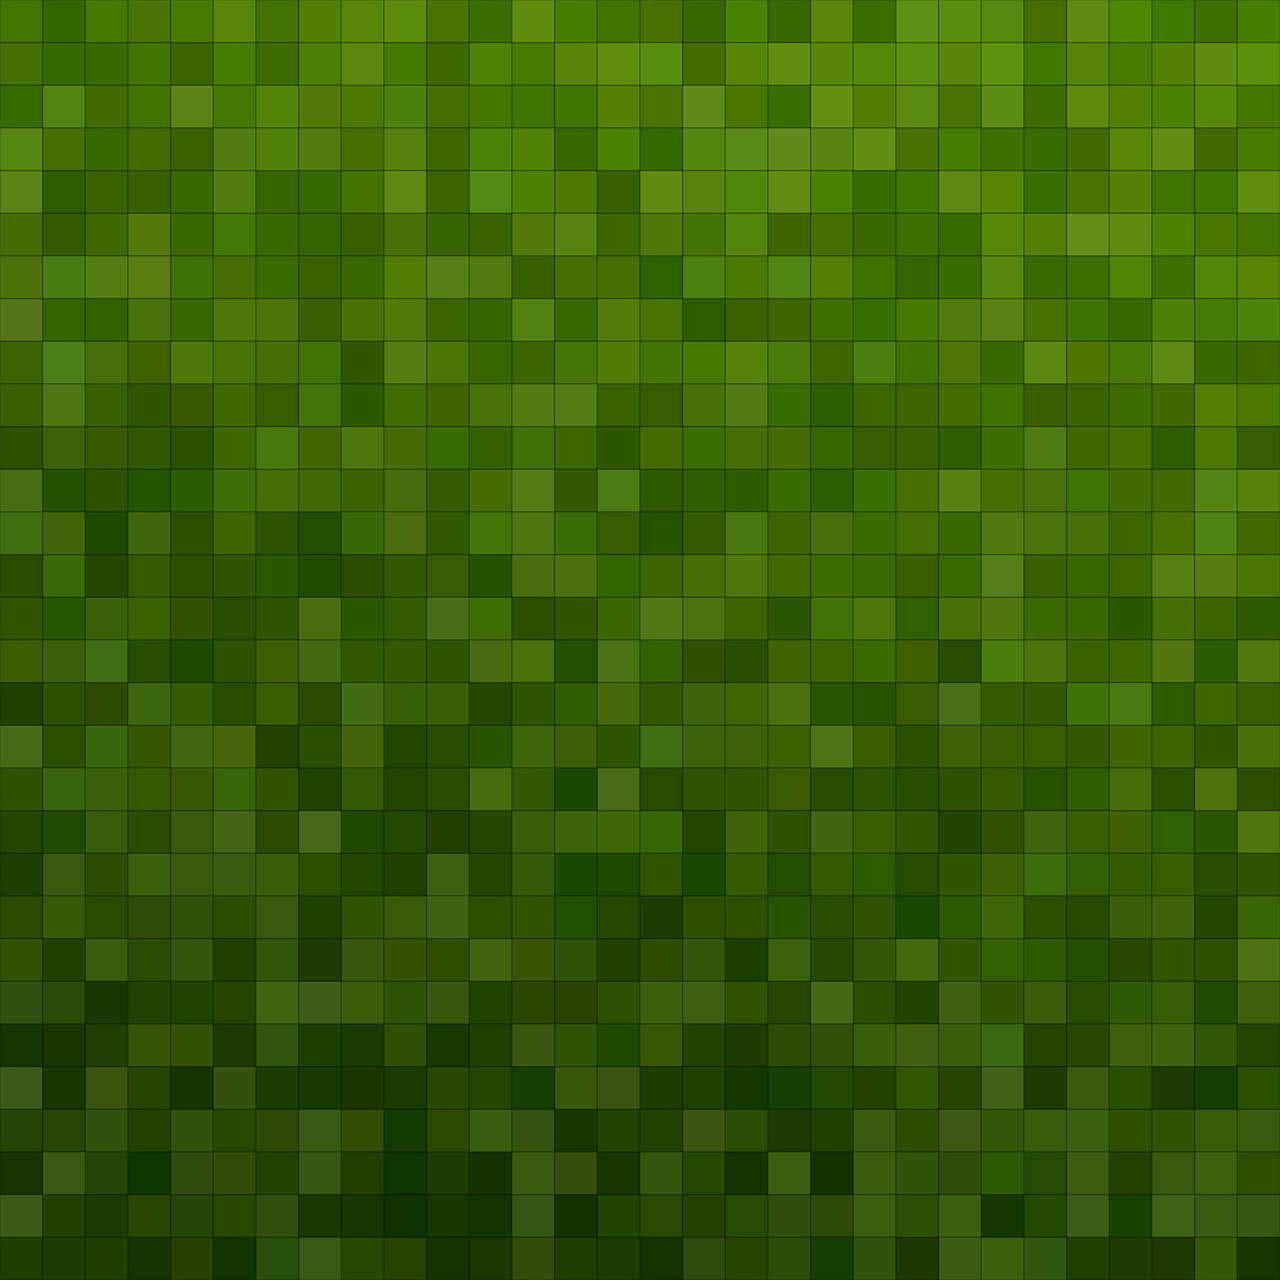
\includegraphics[width=0.25\textwidth]{cover.png}}
\author{I am the BATMAN}
\date{May, 2021}
\maketitle

%%-----------------------------------------------------------
%% Blank Page
%%-----------------------------------------------------------
%-----------------------------------------------------------
% Blank Page
% Usage: %-----------------------------------------------------------
% Blank Page
% Usage: %-----------------------------------------------------------
% Blank Page
% Usage: \include{blank-page}
%-----------------------------------------------------------
\newpage
\mbox{}
\thispagestyle{plain}
\newpage
%-----------------------------------------------------------
\newpage
\mbox{}
\thispagestyle{plain}
\newpage
%-----------------------------------------------------------
\newpage
\mbox{}
\thispagestyle{plain}
\newpage

%-----------------------------------------------------------
% Dedicated TO
%-----------------------------------------------------------
\newpage
\thispagestyle{plain}
\vspace*{1cm}
\begin{center}
{\Large DEDICATION}
\end{center}
\vspace*{1cm}

\begin{center}
To YOUR parents bro, always.
\end{center}

%%-----------------------------------------------------------
%% Blank Page
%%-----------------------------------------------------------
%-----------------------------------------------------------
% Blank Page
% Usage: %-----------------------------------------------------------
% Blank Page
% Usage: %-----------------------------------------------------------
% Blank Page
% Usage: \include{blank-page}
%-----------------------------------------------------------
\newpage
\mbox{}
\thispagestyle{plain}
\newpage
%-----------------------------------------------------------
\newpage
\mbox{}
\thispagestyle{plain}
\newpage
%-----------------------------------------------------------
\newpage
\mbox{}
\thispagestyle{plain}
\newpage

%-----------------------------------------------------------
% Prologue
%-----------------------------------------------------------
\newpage
\thispagestyle{plain}
\begin{center}
{\Large PROLOGUE}
\end{center}
\vspace*{0.5cm}
    


Lorem ipsum dolor sit amet, consectetur adipiscing elit, sed do eiusmod tempor incididunt ut labore et dolore magna aliqua. Ut enim ad minim veniam, quis nostrud exercitation ullamco laboris nisi ut aliquip ex ea commodo consequat. Duis aute irure dolor in reprehenderit in voluptate velit esse cillum dolore eu fugiat nulla pariatur. Excepteur sint occaecat cupidatat non proident, sunt in culpa qui officia deserunt mollit anim id est laborum

%%-----------------------------------------------------------
%% Blank Page
%%-----------------------------------------------------------
%-----------------------------------------------------------
% Blank Page
% Usage: %-----------------------------------------------------------
% Blank Page
% Usage: %-----------------------------------------------------------
% Blank Page
% Usage: \include{blank-page}
%-----------------------------------------------------------
\newpage
\mbox{}
\thispagestyle{plain}
\newpage
%-----------------------------------------------------------
\newpage
\mbox{}
\thispagestyle{plain}
\newpage
%-----------------------------------------------------------
\newpage
\mbox{}
\thispagestyle{plain}
\newpage

%-----------------------------------------------------------
% Lists
%-----------------------------------------------------------
\renewcommand{\listtablename}{Custom Table Index Name}  % Customizing Table Index Name
\renewcommand{\tablename}{Custom Table Name}            % Customizing Table Names
\tableofcontents
\listoffigures
\listoftables

%%-----------------------------------------------------------
%% Blank Page
%%-----------------------------------------------------------
%-----------------------------------------------------------
% Blank Page
% Usage: %-----------------------------------------------------------
% Blank Page
% Usage: %-----------------------------------------------------------
% Blank Page
% Usage: \include{blank-page}
%-----------------------------------------------------------
\newpage
\mbox{}
\thispagestyle{plain}
\newpage
%-----------------------------------------------------------
\newpage
\mbox{}
\thispagestyle{plain}
\newpage
%-----------------------------------------------------------
\newpage
\mbox{}
\thispagestyle{plain}
\newpage

%-----------------------------------------------------------
% Nomenclature
%-----------------------------------------------------------
\newpage
\thispagestyle{plain}
\section*{NOMENCLATURE}
    \label{sec:nomenclature}
\vspace*{1cm}

Basic nomenclature used in the document.\newline
\vspace*{2cm}

% Image by Darwis Alwan - https://pixabay.com/users/darwisalwan-2057348/?utm_source=link-attribution&amp;utm_medium=referral&amp;utm_campaign=image&amp;utm_content=3400005
\begin{figure}[thpb]
    \centering
    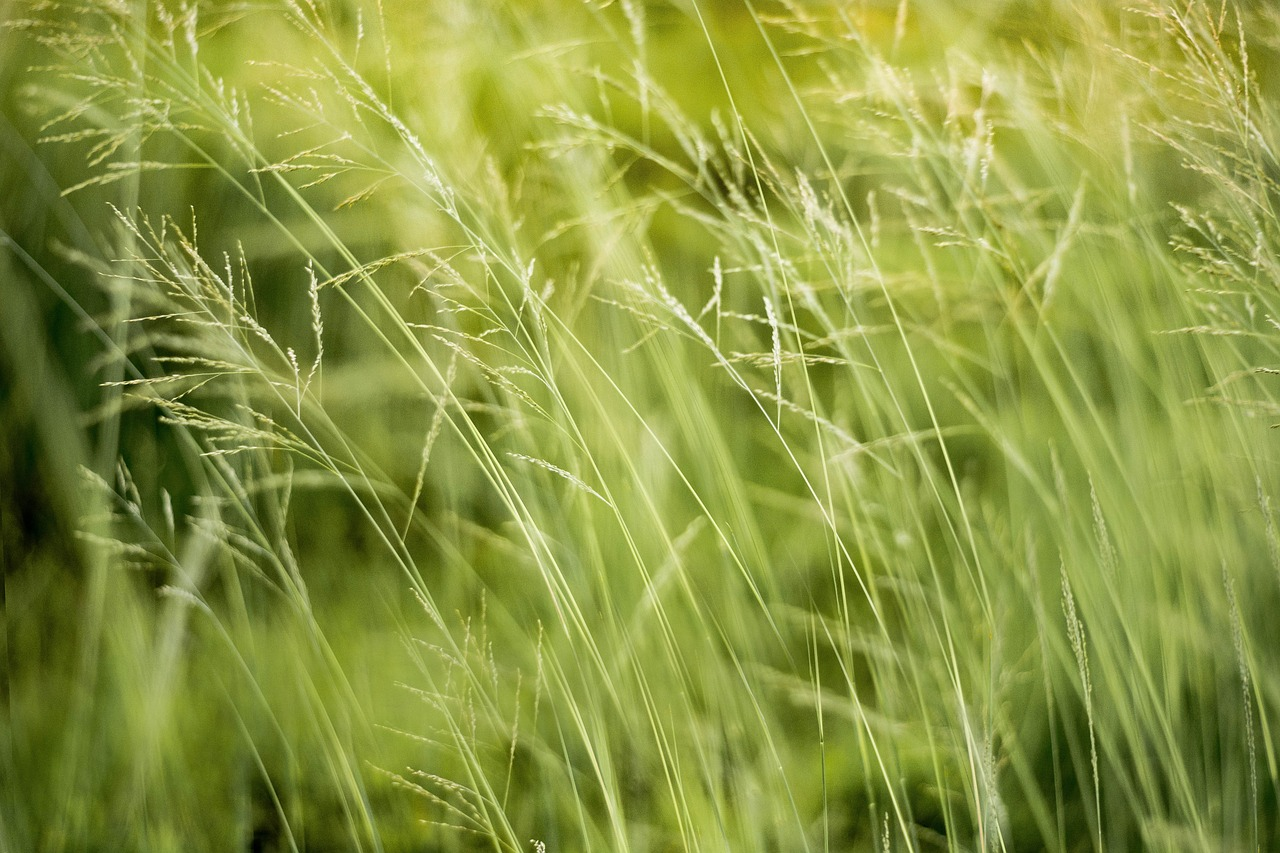
\includegraphics[width=0.5\textwidth]{nomenclature/nomenclature_img_1.jpg}
    \caption[Basic Nomenclature]{\bf{Basic Nomenclature}}
	\label{fig:nomenclature}
\end{figure}

%-----------------------------------------------------------
% Blank Page
%-----------------------------------------------------------
%-----------------------------------------------------------
% Blank Page
% Usage: %-----------------------------------------------------------
% Blank Page
% Usage: %-----------------------------------------------------------
% Blank Page
% Usage: \include{blank-page}
%-----------------------------------------------------------
\newpage
\mbox{}
\thispagestyle{plain}
\newpage
%-----------------------------------------------------------
\newpage
\mbox{}
\thispagestyle{plain}
\newpage
%-----------------------------------------------------------
\newpage
\mbox{}
\thispagestyle{plain}
\newpage

%-----------------------------------------------------------
% Chapters
%-----------------------------------------------------------
\chapter[Chapter 1: One]{Chapter 1: One \footnote{This chapter is based on \cite{einstein}, \cite{latexcompanion} and \cite{knuthwebsite}.}}
\label{chap:chapter_1} 

\section{Introduction}

\index{Lorem ipsum dolor sit amet}, consectetur adipiscing elit, sed do eiusmod tempor incididunt ut labore et dolore magna aliqua. Ut enim ad minim veniam, quis nostrud exercitation ullamco laboris nisi ut aliquip ex ea commodo consequat. Duis aute irure dolor in reprehenderit in voluptate velit esse cillum dolore eu fugiat nulla pariatur. Excepteur sint occaecat cupidatat non proident, sunt in culpa qui officia deserunt mollit anim id est laborum.

% Image by Aurélien Barre - https://pixabay.com/users/aurelbzh-3842842/?utm_source=link-attribution&amp;utm_medium=referral&amp;utm_campaign=image&amp;utm_content=6278951"
\begin{figure}[thpb]
    \centering
    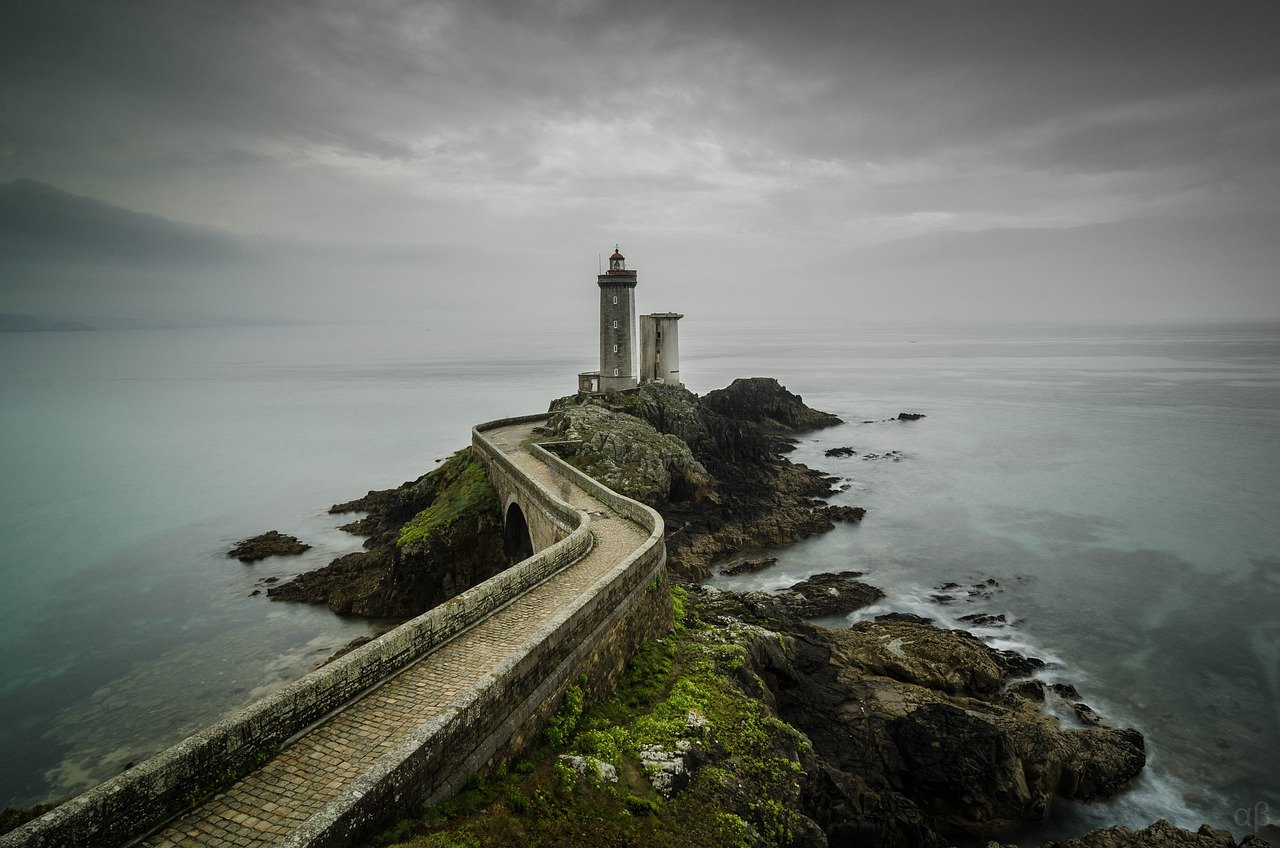
\includegraphics[width=0.75\textwidth]{chapter_1/chapter_1_img_1.jpg}
    \caption[Image 1]{\bf{Image 1}}
    \label{fig:chapt_1_img_1}
\end{figure}

Lorem ipsum dolor sit amet, consectetur adipiscing elit, sed do eiusmod tempor incididunt ut labore et dolore magna aliqua. Ut enim ad minim veniam, quis nostrud exercitation ullamco laboris nisi ut aliquip ex ea commodo consequat. Duis aute irure dolor in reprehenderit in voluptate velit esse cillum dolore eu fugiat nulla pariatur. Excepteur sint occaecat cupidatat non proident, sunt in culpa qui officia deserunt mollit anim id est laborum.\newline

You can check information on table \ref{tab:chaper_1_table_1} 

\begin{table}[thpb]
\begin{center}
\begin{tabular}{l l}
ROW 1&COL 1\\
ROW 2&COL 1\\
ROW 3&COL 1\\
ROW 4&COL 1\\
\end{tabular}
\caption[Chapter 1 Table 1]{\bf{Chapter 1 Table 1}}
\label{tab:chaper_1_table_1}
\end{center}
\end{table}

Lorem ipsum dolor sit amet, consectetur adipiscing elit, sed do eiusmod tempor incididunt ut labore et dolore magna aliqua. Ut enim ad minim veniam, quis nostrud exercitation ullamco laboris nisi ut aliquip ex ea commodo consequat. Duis aute irure dolor in reprehenderit in voluptate velit esse cillum dolore eu fugiat nulla pariatur. Excepteur sint occaecat cupidatat non proident, sunt in culpa qui officia deserunt mollit anim id est laborum.


\chapter[Chapter 2: Two]{Chapter 2: Two \footnote{This chapter is based on \cite{einstein}, \cite{latexcompanion} and \cite{knuthwebsite}.}}
\label{chap:chapter_2} 

\section{Introduction}

\index{Lorem ipsum dolor sit amet}, consectetur adipiscing elit, sed do eiusmod tempor incididunt ut labore et dolore magna aliqua. Ut enim ad minim veniam, quis nostrud exercitation ullamco laboris nisi ut aliquip ex ea commodo consequat. Duis aute irure dolor in reprehenderit in voluptate velit esse cillum dolore eu fugiat nulla pariatur. Excepteur sint occaecat cupidatat non proident, sunt in culpa qui officia deserunt mollit anim id est laborum.
% Image by salofoto - https://pixabay.com/users/salofoto-11386676/?utm_source=link-attribution&amp;utm_medium=referral&amp;utm_campaign=image&amp;utm_content=6274156
\begin{figure}[thpb]
    \centering
    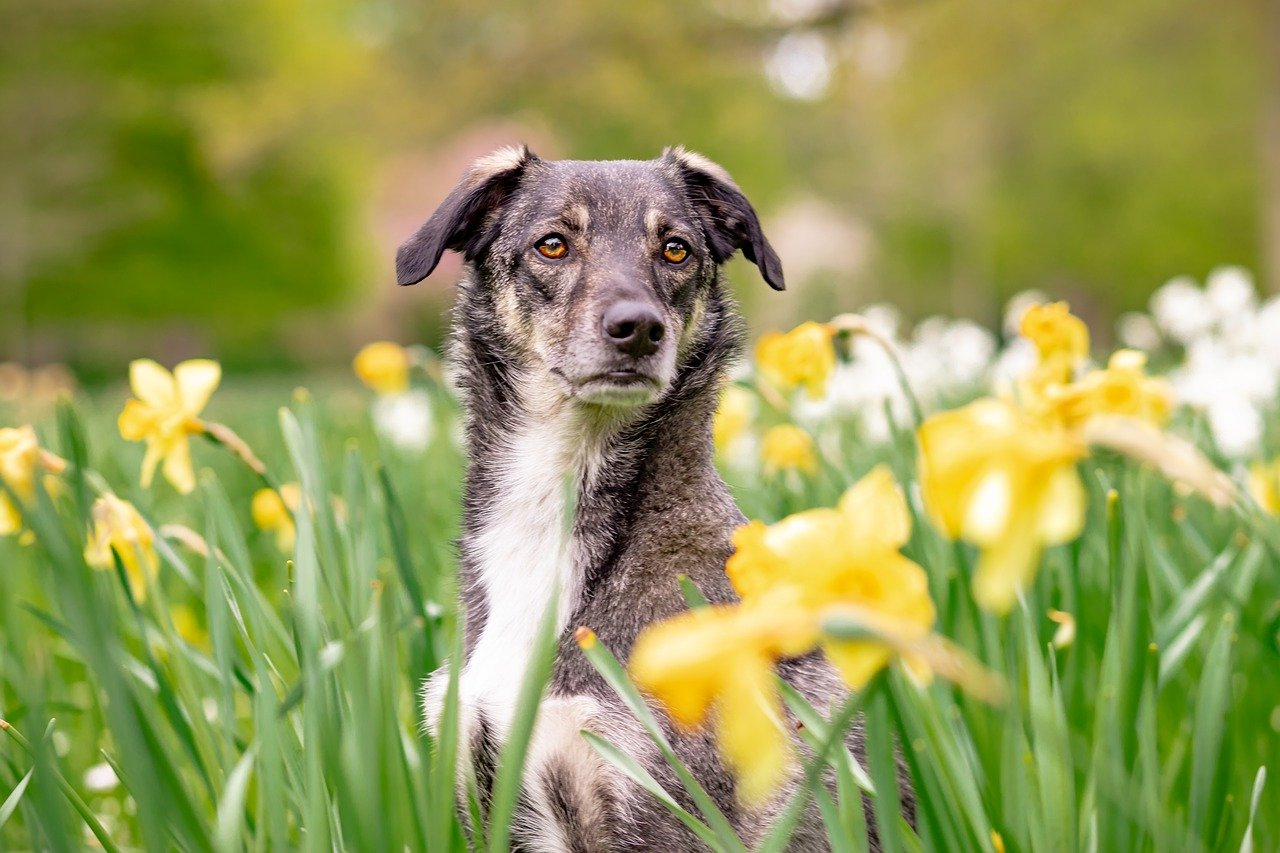
\includegraphics[width=0.75\textwidth]{chapter_2/chapter_2_img_1.jpg}
    \caption[Image 1]{\bf{Image 1}}
    \label{fig:chapt_1_img_1}
\end{figure}

Lorem ipsum dolor sit amet, consectetur adipiscing elit, sed do eiusmod tempor incididunt ut labore et dolore magna aliqua. Ut enim ad minim veniam, quis nostrud exercitation ullamco laboris nisi ut aliquip ex ea commodo consequat. Duis aute irure dolor in reprehenderit in voluptate velit esse cillum dolore eu fugiat nulla pariatur. Excepteur sint occaecat cupidatat non proident, sunt in culpa qui officia deserunt mollit anim id est laborum.\newline

You can check information on table \ref{tab:chaper_2_table_1} 

\begin{table}[thpb]
\begin{center}
\begin{tabular}{l l}
ROW 1&COL 1\\
ROW 2&COL 1\\
ROW 3&COL 1\\
ROW 4&COL 1\\
\end{tabular}
\caption[Chapter 2 Table 1]{\bf{Chapter 2 Table 1}}
\label{tab:chaper_2_table_1}
\end{center}
\end{table}

Lorem ipsum dolor sit amet, consectetur adipiscing elit, sed do eiusmod tempor incididunt ut labore et dolore magna aliqua. Ut enim ad minim veniam, quis nostrud exercitation ullamco laboris nisi ut aliquip ex ea commodo consequat. Duis aute irure dolor in reprehenderit in voluptate velit esse cillum dolore eu fugiat nulla pariatur. Excepteur sint occaecat cupidatat non proident, sunt in culpa qui officia deserunt mollit anim id est laborum.

%\include{chapter_3}
%\include{chapter_4}
%\include{chapter_5}
%\include{chapter_6}
% ... and so on

%-----------------------------------------------------------
% Appendix
%-----------------------------------------------------------
\appendix
\chapter[Appendix 1]{Appendix 1}
\label{app:appendix_1}

Lorem ipsum dolor sit amet, consectetur adipiscing elit, sed do eiusmod tempor incididunt ut labore et dolore magna aliqua. Ut enim ad minim veniam, quis nostrud exercitation ullamco laboris nisi ut aliquip ex ea commodo consequat. Duis aute irure dolor in reprehenderit in voluptate velit esse cillum dolore eu fugiat nulla pariatur. Excepteur sint occaecat cupidatat non proident, sunt in culpa qui officia deserunt mollit anim id est laborum.

\chapter[Appendix 2]{Appendix 2}
\label{app:appendix_2}

Lorem ipsum dolor sit amet, consectetur adipiscing elit, sed do eiusmod tempor incididunt ut labore et dolore magna aliqua. Ut enim ad minim veniam, quis nostrud exercitation ullamco laboris nisi ut aliquip ex ea commodo consequat. Duis aute irure dolor in reprehenderit in voluptate velit esse cillum dolore eu fugiat nulla pariatur. Excepteur sint occaecat cupidatat non proident, sunt in culpa qui officia deserunt mollit anim id est laborum.

%\include{appendix_3}
%\include{appendix_4}
%\include{appendix_5}
%\include{appendix_6}
% ... and so on
\pagestyle{plain}
\appendix
\section*{ACRONYMS}
\label{appendix:acronyms}
\vspace*{1cm}

\begin{longtable}{l|l}
3G&Third Generation\\
&Third Generation Partnership Project\\
WTF&What The Frack\\
\end{longtable}


%-----------------------------------------------------------
% Alphabetic Index - Yo sure ?
%-----------------------------------------------------------

%\printindex % Youn only have to add command: \index{key} to the desired key reference

%-----------------------------------------------------------
% Bibliography
%-----------------------------------------------------------
\bibliographystyle{IEEEtranS}
\bibliography{bibliography}
\end{document}
